\chapter{Project Context and Objectives}
\label{chap:Project_Context_and_Objectives}

\section*{Introduction}
Dans cette partie, on va parler du contexte du projet, la
problématique qu’il résout ainsi que l’objectif du projet.


\vspace{0.5cm}
\section{Cadre Général du projet}
\subsection{General Context}

Today's world is witnessing a massive acceleration in the pace of digital transformation, opening up broad horizons for automating various sectors to become more efficient and effective. However, the legal and administrative sector, particularly in Morocco, still relies heavily on traditional methods. This makes the process of accessing accurate legal information or administrative consultations complex, expensive, and highly time-and-effort consuming.

As first-year engineering students in the "Advanced Software Engineering for Digital Services" (ASEDS) program at the National Institute of Posts and Telecommunications (INPT), we have acquired a solid academic foundation encompassing software engineering, advanced databases, and the development of complex systems[cite: 2]. Building on this foundation, and amidst the current artificial intelligence revolution, we identified an exceptional opportunity to leverage these modern technologies (specifically in the LegalTech domain) to modernize this sector, making it easier for individuals to access the information they need seamlessly and reliably.


\subsection{Problem Statement}

Despite the urgent need to digitize the legal sector, integrating artificial intelligence into this field in Morocco faces several technical and economic challenges, which can be summarized in the following points:

\begin{itemize}
    \item \textbf{High Cost and Lack of Automation:} The legal field lacks automation, making legal consultations prohibitively expensive. Legal consultants charge substantial fees, leaving the average user with a dilemma: either spend long hours in manual web searches that may yield no results, or pay exorbitant amounts for a simple answer.
    
    \item \textbf{Shortcomings of Global Language Models (Risk of Hallucination):} Despite the immense capabilities of Large Language Models (LLMs), they are primarily trained on foreign data and lack deep knowledge of Moroccan legal sources. Consequently, when asked about a specific Moroccan legal procedure, they often fall into the trap of "hallucination," providing completely fabricated and incorrect answers.
    
    \item \textbf{Data Extraction Challenge (Document Format):} Moroccan legal documents and administrative circulars are rarely available in smooth digital formats. Instead, they are typically scanned PDF files containing tables, stamps, and signatures. Classical text extraction (OCR) tools fail to process these files and extract information from them.
    
    \item \textbf{Linguistic and Semantic Barrier:} Most documents are drafted in formal legal Arabic. Processing this type of text requires a powerful Embedding Model trained specifically on the Arabic language to conduct accurate semantic searches.
\end{itemize}


\subsection{Project Objectives}

Faced with these challenges, our project aims to build an integrated digital platform by achieving the following primary and secondary objectives:

\begin{itemize}
    \item Conduct a precise needs analysis and prepare the project's specifications document (Cahier des charges).
    \item Select the best technologies and programming languages (Tech Stack) most suited for building the project.
    \item Build a Retrieval-Augmented Generation (RAG) system: To minimize hallucination and force the AI to extract answers exclusively from approved Moroccan sources and documents.
    \item Build advanced pipelines.
    \item Select the best Embedding Model.
    \item Select the best Optical Character Recognition (OCR) model, relying on an intelligent AI-powered model, which includes:
    \begin{itemize}
        \item Converting PDF documents into high-quality images.
        \item Sending these images to our model along with a prompt specifically designed and tailored to handle this type of document.
        \item Saving the outputs in the database, utilizing them in the retrieving process, and enabling the system to handle these documents highly efficiently.
    \end{itemize}
    
    \item Build the User Interface, which includes the following functionalities:
    \begin{itemize}
        \item Enabling the user to communicate directly with the Large Language Model (LLM) powered by the RAG system.
        \item Allowing the user to send and upload their own documents to the Chatbot.
        \item Empowering the user to create and draft documents using LaTeX via code, prompting the Chatbot to generate them using ready-made templates, or making modifications to their own files.
    \end{itemize}
    
    \item Build a secure Authentication System for user login.
    \item Secure the project to protect user data and their uploaded files.
    \item Build an optimized database.
    \item Build a Log System.
    \item Optimize the system to support the largest possible number of concurrent users while reducing operational costs.
    \item Conduct Testing and Quality Assurance (QA) operations to ensure the platform is bug-free.
    \item Project Deployment.
\end{itemize}

\newpage
\section{Conduite de projet}

\subsection{Méthodologie adoptée}

\subsubsection{Méthode Scrum}

Scrum est un schéma d'organisation de développement de produits complexes. Il est défini par ses créateurs comme un « cadre de travail holistique itératif qui se concentre sur les buts communs en livrant de manière productive et créative des produits de la plus grande valeur possible ». Scrum est considéré comme un groupe de pratiques répondant pour la plupart aux préconisations du Manifeste Agile.

\begin{figure}[htbp]
    \centering
    \IfFileExists{Figures/1.png}{
        
\includegraphics[width=0.8\textwidth]{Figures/1.png}
    }{
        \framebox[12cm]{\rule{0pt}{6cm} \textbf{Image manquante: Figures/1.png}}
    }
    \caption{Schéma explicatif de scrum}
\end{figure}

Pour mettre en place un projet en suivant les bonnes pratiques SCRUM, il nous faut :

\begin{itemize}
    \item Une équipe responsable et autonome qui peut pallier les éventuels changements d'un client trop indécis.
    \item Une organisation du travail par une série de « sprints » : des itérations courtes de 2 à 4 semaines au plus, pour permettre des interventions rapides en cas de problèmes.
    \item Une définition des exigences : On devra rassembler les éléments à mettre en œuvre dans une liste qu'on appelle « Backlog du produit ».
\end{itemize}

\subsubsection{Rôles dans SCRUM}

Scrum définit les rôles principaux suivants :

\begin{enumerate}[label=\arabic*)]
    \item Le Product Owner : C'est le directeur du produit, représentant du client et de ses attentes. Il est obligatoire qu'il soit disponible pour répondre aux questions.
    \item Le Scrum Master : C'est celui qui est chargé de veiller sur l'application des valeurs SCRUM. Il protège aussi l'équipe de tout élément perturbateur extérieur et résout les problèmes.
    \item L'équipe : elle est autonome et s'auto-gère. Pas de concept de hiérarchie, et toutes les décisions sont discutés et prises ensemble.
\end{enumerate}

Ces trois parties s'organisent entre eux pour animer les événements SCRUM suivants :

\begin{itemize}
    \item Les Sprints : c'est le découpage d'un projet en boîte de temps, le sprint commence après la fin du sprint précédent et a une durée de deux à quatre semaines.
    \item Le Sprint Planning : c'est la planification du sprint courant, elle se fait au début de chaque sprint c'est là où sont choisis les fonctionnalités ou User stories à travailler durant la période du sprint.
    \item Le Sprint Exécution : C'est l'exécution du travail planifié. Il contient optionnellement une phase de conception suivi d'une phase de développement.
    \item Le Sprint Review et rétrospective : c'est une chance de se remettre en question de revenir sur ce qui a été effectué et ce qui peut être amélioré à la fin de chaque sprint.
    \item Le Product Backlog Grooming : puisque l'agile permet le changement, le Product Backlog est sujet à un changement qui se fait de manière continue après la fin du sprint.
\end{itemize}

\subsection{Répartition des rôles}

Durant ce stage, notre équipe se composait de :

Durant ce projet, en raison de la taille réduite de notre équipe, il n'y avait pas littéralement un Scrum Master dédié à plein temps. C'est pourquoi nous avons essayé de simuler au mieux la méthodologie Scrum en adaptant les rôles de manière collaborative 


\subsection{Outils de collaboration}

\begin{itemize}
    \item \textbf{Utilisation de whatsapp}
\end{itemize}

En général, nous utilisions whatsapp pour effectuer quatre types de réunions durant notre project :

\begin{itemize}
    \item Des réunions quotidiennes qui permettaient aux membres de l'équipe de partager ce qu'ils ont fait la veille, et de discuter ce qu'il y a à faire.
    \item Des réunions du Peer-Programming : qui permettaient aux membres de l'équipe de faire de la conception et de résoudre éventuellement des problèmes techniques assez complexes.
    
    \item Réunion de présentation du produit : c'est une seule présentation qu'on avait à faire à la fin de notre project, durant laquelle on a fait une démonstration de la solution.
\end{itemize}



\begin{figure}[htbp]
    \centering
    \IfFileExists{Figures/2.png}{
        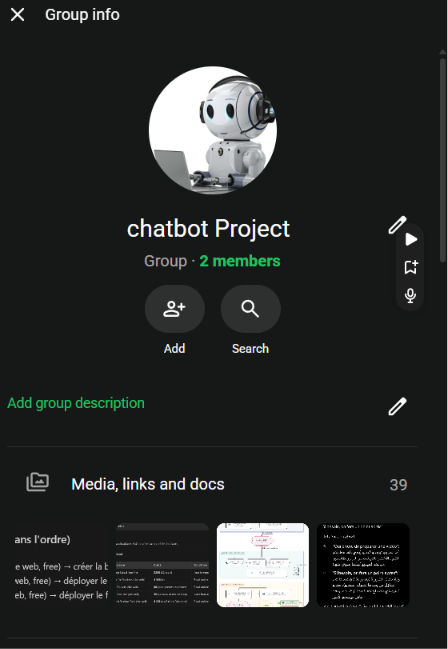
\includegraphics[width=0.9\textwidth]{Figures/2.png}
    }{
        \framebox[12cm]{\rule{0pt}{6cm} \textbf{Image manquante: Figures/2.png}}
    }
    \caption{Capture d'écran dans WhatsApp}
\end{figure}
\begin{itemize}
    \item \textbf{Gestion du code source avec Git et GitHub}
\end{itemize}

Nous avons utilisé \textbf{Git} et \textbf{GitHub} pour centraliser notre code en ligne, permettant à l'équipe de suivre et d'évaluer la dernière version du projet. Nous avons adopté une stratégie de \textbf{Branching} et \textbf{Merge} après validation. 

De plus, chaque \textbf{Commit} a été soigneusement rédigé pour décrire précisément le travail accompli et la prochaine étape , garantissant ainsi une traçabilité totale comme l'illustre la figure ci-dessous :

\begin{figure}[htbp]
    \centering
    \IfFileExists{Figures/3.png}{
        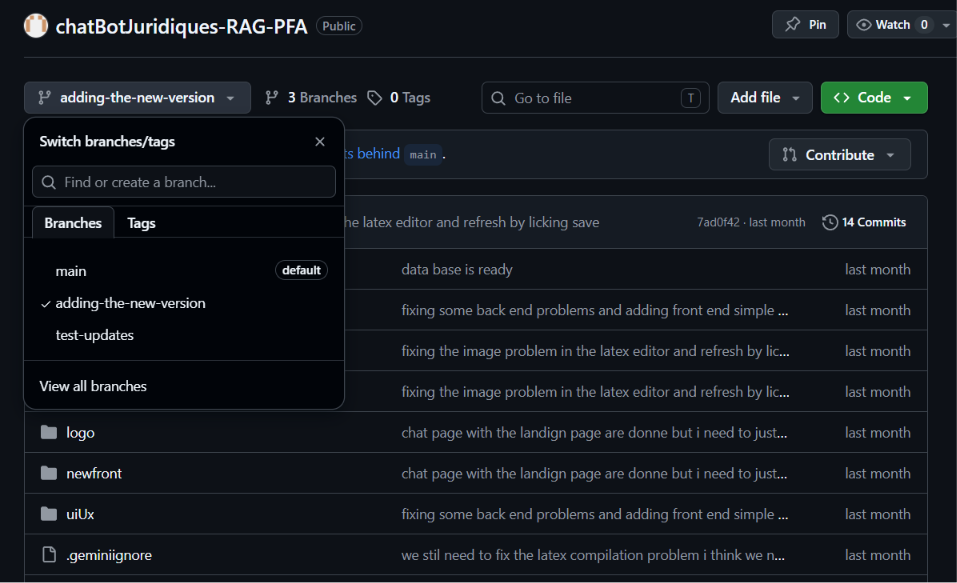
\includegraphics[width=0.9\textwidth]{Figures/3.png}
    }{
        \framebox[12cm]{\rule{0pt}{5cm} \textbf{Image manquante: Figures/3.png (Capture des Commits)}}
    }
    \caption{Historique des commits et messages de suivi sur GitHub}
\end{figure}

\section*{Conclusion}
Maintenant, comme on a bien défini le contexte du projet, les problématiques et
finalement les objectifs permettant de mesurer la réussite ou non du projet. On va passer
à la spécification des besoins ainsi que l’analyse et la conception de notre projet.
